Más de 666 millones de personas en el mundo todavía no tienen acceso a la electricidad. En Colombia, cerca del 53\,\% del territorio, contado por municipios, hace parte de las Zonas No Interconectadas (ZNI): municipios, corregimientos y caseríos que no están conectados al Sistema Interconectado Nacional. En estas zonas el 79\,\% de los usuarios recibe energía producida con combustibles fósiles, en su mayoría diésel, y solo el 9\,\% la recibe de fuentes renovables no convencionales.

Donde hay un río o una quebrada cerca, una alternativa son las pico centrales hidroeléctricas, plantas de generación de menos de 5~kW. Con esa potencia no se abastece una ciudad, pero sí viviendas o pequeñas comunidades rurales, con una tecnología sencilla, de bajo costo y que no necesita combustible. La pieza central de estas plantas es la turbina: una rueda que gira cuando un chorro de agua golpea las pequeñas cucharas, llamadas cangilones, ubicadas en su borde, y que a su vez mueve un generador eléctrico. Dos de las turbinas que se usan en este rango son la Pelton y la Turgo (Lakdawala, 2025).

La pregunta práctica es qué tanto de la energía que trae el agua termina convertida en energía útil en el eje de la turbina. Esa proporción se llama eficiencia hidráulica y, con la misma cantidad de agua, una turbina más eficiente genera más electricidad. Por eso interesa saber qué decisiones de diseño la aumentan: qué tipo de turbina usar, si poner uno o dos chorros de agua y cómo ubicar la boquilla por la que sale cada chorro (su diámetro, su ángulo y su distancia a la rueda). En términos estadísticos, el problema consiste en explicar una variable respuesta continua, la eficiencia, a partir de cinco variables explicativas, que es justamente lo que permite hacer el análisis de regresión.

Lakdawala (2025) estudiaron esta pregunta con un experimento de laboratorio. Construyeron dos turbinas pequeñas, una Pelton y una Turgo, del mismo tamaño y con el mismo disco central; como se ve en la Figura~\ref{fig:rodetes}, la única diferencia entre ellas es la forma de los cangilones.

\begin{figure}[H]
\centering
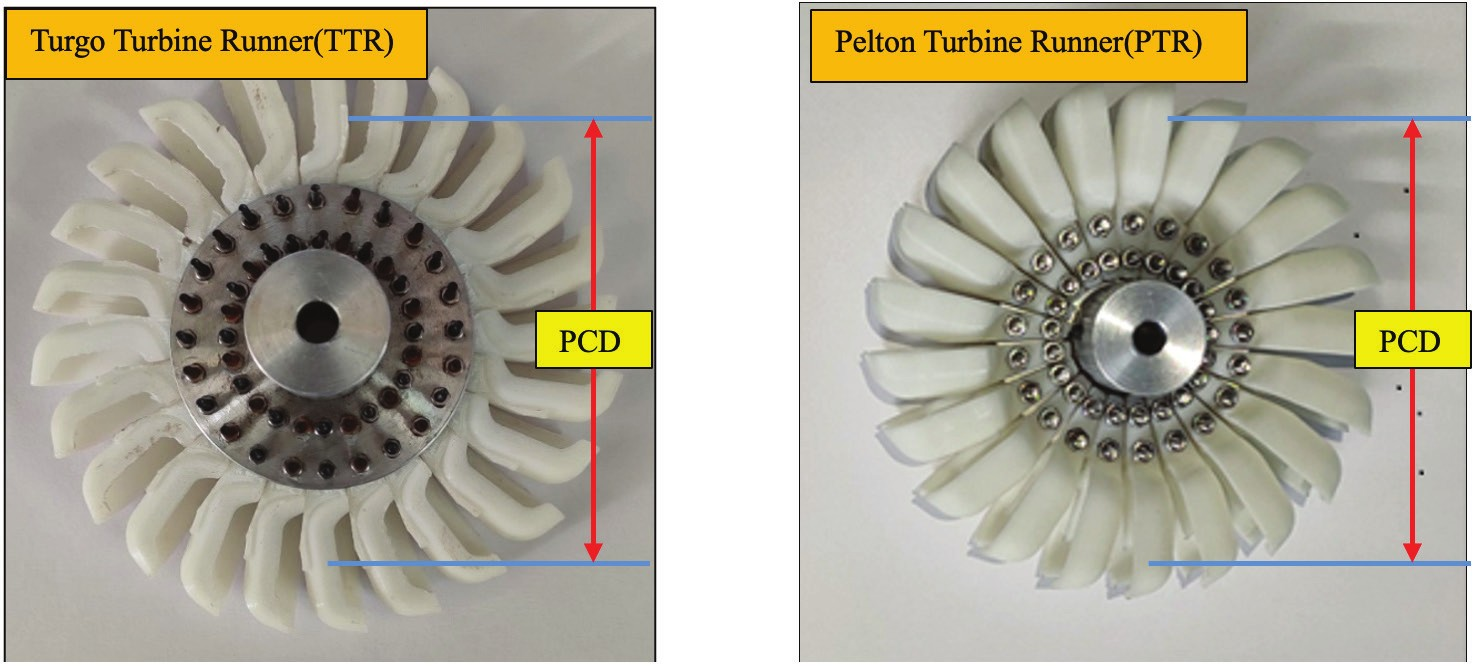
\includegraphics[width=0.85\textwidth]{Articulo_LaTeX/Figs/lakdawala_rodetes.jpg}
\caption{Las dos turbinas del experimento, Turgo (izquierda) y Pelton (derecha), vistas desde arriba. La flecha roja marca el diámetro de la circunferencia donde el chorro golpea los cangilones, que es el mismo en las dos. Fuente: (Lakdawala, 2025).}
\label{fig:rodetes}
\end{figure}

Las turbinas se probaron en el banco de pruebas de la Figura~\ref{fig:montaje}, con la misma altura de agua en todos los ensayos. Una bomba lleva el agua hasta las boquillas, el chorro hace girar la rueda y, en cada ensayo, se midieron el caudal de agua, la velocidad de giro de la rueda y la fuerza de giro en el eje; con esas tres mediciones se calculó la eficiencia. Los detalles técnicos del montaje no son necesarios para el análisis estadístico, pero los términos que aparecen en el artículo original se explican en el glosario del Apéndice~\ref{sec:glosario}.

\begin{figure}[H]
\centering
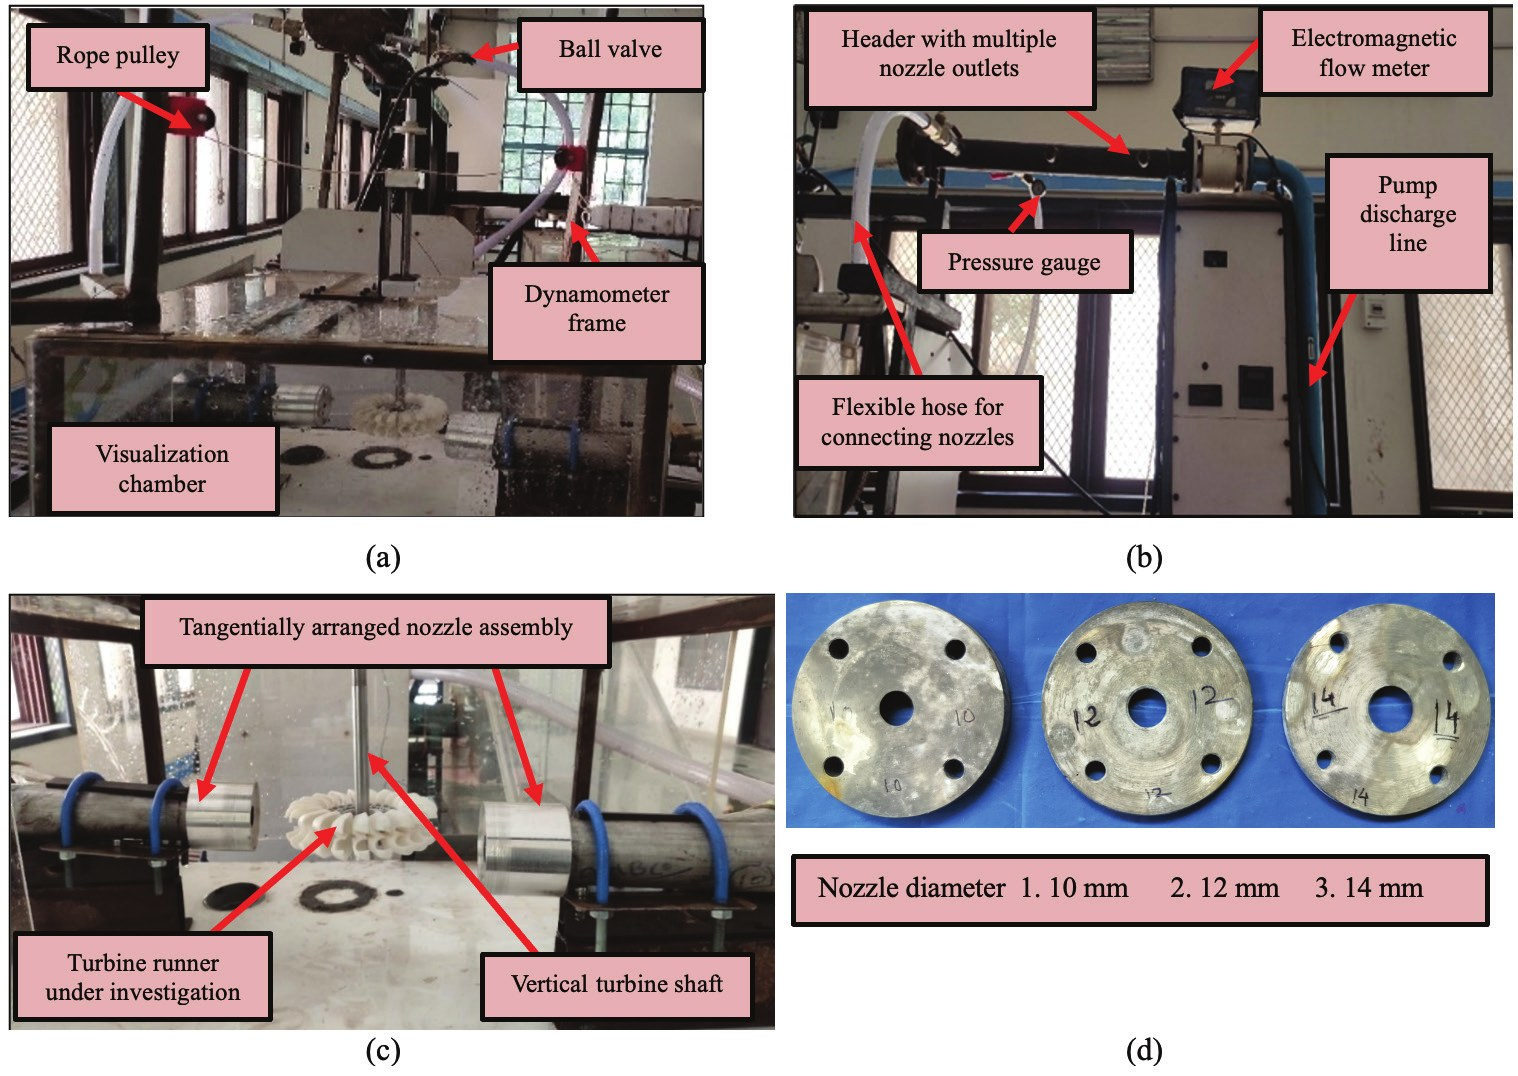
\includegraphics[width=0.9\textwidth]{Articulo_LaTeX/Figs/lakdawala_montaje.jpg}
\caption{Banco de pruebas: (a) sistema para medir la fuerza de giro en el eje, (b) tubería con el medidor de caudal, (c) las dos boquillas frente a la turbina y (d) las tres placas que fijan el diámetro de la boquilla (10, 12 y 14~mm). Fuente: (Lakdawala, 2025).}
\label{fig:montaje}
\end{figure}

En cada uno de los 80 ensayos, llamados corridas, los investigadores fijaron cinco variables: el tipo de turbina (Pelton o Turgo), el número de boquillas (una o dos) y tres características de la boquilla, que son su diámetro (10, 12 o 14~mm), su ángulo y su distancia a la rueda. La Figura~\ref{fig:chorro} muestra qué significan las dos últimas. El ángulo indica qué tan de frente llega el chorro a la rueda: 90° es perpendicular y 92.5° y 95° son desviaciones pequeñas. La distancia es el recorrido del chorro entre la boquilla y la rueda, que se varió entre 40 y 60~mm.

\begin{figure}[H]
\centering
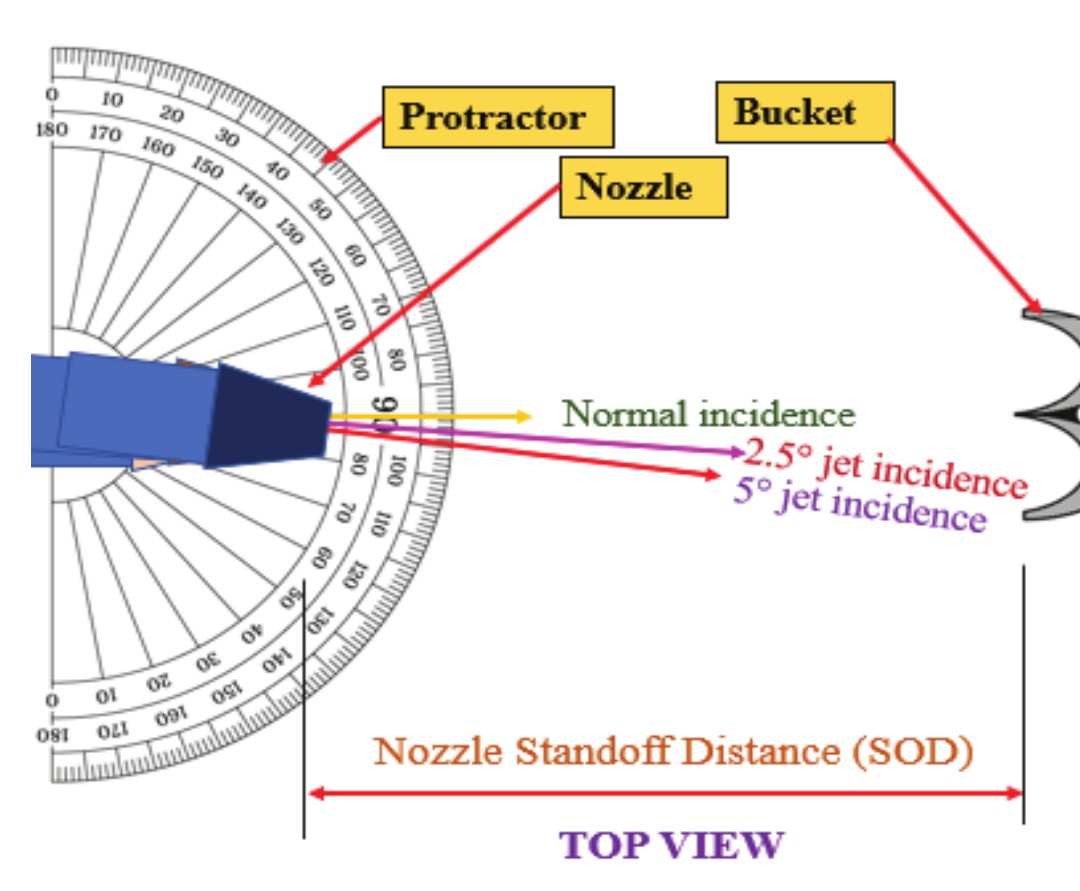
\includegraphics[width=0.55\textwidth]{Articulo_LaTeX/Figs/lakdawala_chorro.jpg}
\caption{Vista desde arriba de la boquilla y un cangilón: ángulo del chorro (perpendicular, desviado 2.5° y desviado 5°) y distancia entre la boquilla y el cangilón (\textit{Nozzle Standoff Distance}). Fuente: (Lakdawala, 2025).}
\label{fig:chorro}
\end{figure}

Las combinaciones de valores no se escogieron al azar. Los autores usaron un diseño central compuesto, un tipo de diseño experimental pensado para ajustar modelos de regresión con términos cuadráticos usando pocas corridas. Por eso cada variable numérica toma solo tres valores (bajo, medio y alto) y varias corridas se repiten en el punto central, con las tres variables en su valor medio. Con estos datos, los autores ajustaron un modelo de regresión cuadrático y buscaron la combinación de variables que maximiza la eficiencia.

En este trabajo se usan los datos publicados por (Lakdawala, 2025) para estudiar, con las herramientas del análisis de regresión, cómo se relaciona la eficiencia hidráulica con las cinco variables. Esta parte presenta la descripción de los datos y el análisis exploratorio, que orientan la construcción del modelo. Todos los cálculos y gráficos se hicieron en R con los paquetes \textsf{ggplot2} y \textsf{GGally}, y el código está en el repositorio indicado en la sección de disponibilidad de datos.
